\section{Temporäres Backend für die Mobile Anwendung}
\setauthor{Antonio Peric}

\subsection{IntelliJ Projekt}
\setauthor{Antonio Peric} 
In der vorliegenden Arbeit wurde ein temporäres Backend mithilfe der Technologieumgebung IntelliJ und der Programmiersprache Java entwickelt. Bei der Umsetzung wurde besonderes Augenmerk auf eine präzise Definition der einzelnen Entitäten, eine klare Setzung der Attribute sowie eine sorgfältige Pflege der Beziehungen zwischen den Entitäten gelegt.
\newline
\newline
Zu Beginn des Entwicklungsprozesses wurde die Funktionalität des temporären Backends genau spezifiziert und in mehrere Entitäten aufgeteilt. Anschließend wurden für jede Entität ihre Eigenschaften und Attribute definiert, um eine klare Struktur und einheitliche Verarbeitung innerhalb des Systems zu gewährleisten.
\newline
\newline
Im weiteren Verlauf der Entwicklung wurden die Beziehungen zwischen den einzelnen Entitäten gepflegt und mit Hilfe von Referenzschlüsseln miteinander verknüpft. Hierbei wurde darauf geachtet, dass die Verknüpfungen korrekt und eindeutig sind, um eine reibungslose Funktionalität des temporären Backends zu gewährleisten.
\newline
\newline
Zusammenfassend lässt sich feststellen, dass das temporäre Backend erfolgreich unter Verwendung der Technologieumgebung IntelliJ und der Programmiersprache Java entwickelt wurde. Durch eine präzise Definition der Entitäten, eine klare Setzung der Attribute und eine sorgfältige Pflege der Beziehungen zwischen den Entitäten konnte eine hohe Qualität und Zuverlässigkeit des Systems erreicht werden.
\newpage
\begin{lstlisting}[language=Java,caption=Entity | Person,label=lst:impl:foo]
    @Entity
    public class Exercise {
        //Attributes
        @Id
        @GeneratedValue(strategy = GenerationType.IDENTITY)
        private long id;
        @Column
        public String name;
        @Column(name = "muscle_group")
        public String muscleGroup;
        //Navigation
        @OneToMany(mappedBy = "exercise", fetch = FetchType.EAGER)
        public Set<WorkoutExercise> workoutExcersices = new HashSet<>();
    }
\end{lstlisting}

\begin{lstlisting}[language=Java,caption=Entity | Trainee,label=lst:impl:foo]
    @Entity
    public class Trainee extends Person{
        //Navigation
        @OneToMany(mappedBy = "trainee", fetch = FetchType.EAGER)
        public Set<Workoutplan> workoutPlanList = new HashSet<>();
    }
\end{lstlisting}

\begin{lstlisting}[language=Java,caption=Entity | Trainer,label=lst:impl:foo]
    @Entity
    public class Trainer extends Person{
        //Navigation
        @OneToMany(mappedBy = "trainer", fetch = FetchType.EAGER)
        public List<Template> templateList;
    }
\end{lstlisting}

\begin{lstlisting}[language=Java,caption=Entity | Template,label=lst:impl:foo]
    @Entity
    public class Template {
        //Attributes
        @Id
        @GeneratedValue(strategy = GenerationType.IDENTITY)
        private long id;
        @Column
        public String name;
        //Navigation
        @ManyToOne
        @JoinColumn(name="trainer_id", nullable=false)
        public Trainer trainer;
    
        @ManyToMany(fetch = FetchType.EAGER)
        @JoinTable(
                name = "Template_Exercise", // name of the association table
                joinColumns = @JoinColumn(name = "template_id"), // foreign key columns
                inverseJoinColumns = @JoinColumn(name = "exercise_id"))
        private Set<Exercise> exercise = new HashSet<>();
    }
\end{lstlisting}
\newpage
\begin{lstlisting}[language=Java,caption=Entity | Workoutplan,label=lst:impl:foo]
    @Entity
    public class Workoutplan {
        //Attributes
        @Id
        @GeneratedValue(strategy = GenerationType.IDENTITY)
        private long id;
        @Column
        public String name;
        //Navigation
        @ManyToOne
        @JoinColumn(name="trainee_id", nullable=false)
        public Trainee trainee;
        @OneToMany(mappedBy = "workoutplan", fetch = FetchType.EAGER)
        public Set<WorkoutExercise> workoutExcersices = new HashSet<>();
    }
\end{lstlisting}

\begin{lstlisting}[language=Java,caption=Entity | WorkoutExersice,label=lst:impl:foo]
    @Entity
    public class WorkoutExercise {
        //Attributes 
        @Id
        @GeneratedValue(strategy = GenerationType.IDENTITY)
        private long id;    
        @Column
        public Integer sets;    
        @Column
        public Double weight;    
        @Column
        public Integer reps;    
        @Column
        public Double time;    
        //Navigation   
        @ManyToOne
        @JoinColumn(name="workoutplan_id", nullable=false)
        public Workoutplan workoutplan;   
        @ManyToOne
        @JoinColumn(name="exercise_id", nullable=false)
        public Exercise exercise;
    }
\end{lstlisting}

\begin{lstlisting}[language=Java,caption=Entity | Exersice,label=lst:impl:foo]
    @Entity
    public class Exercise {
        //Attributes
        @Id
        @GeneratedValue(strategy = GenerationType.IDENTITY)
        private long id;  
        @Column
        public String name;
        @Column(name = "muscle_group")
        public String muscleGroup;
        //Navigation
        @OneToMany(mappedBy = "exercise", fetch = FetchType.EAGER)
        public Set<WorkoutExercise> workoutExcersices = new HashSet<>();
    }
    
\end{lstlisting}

\newpage
\subsection{Packages des IntelliJ Projekts}
\setauthor{Antonio Peric}  

\begin{lstlisting}[language=XML,caption=Dependency | reactive-mysql-client,label=lst:impl:foo]
    <dependency>
      <groupId>io.quarkus</groupId>
      <artifactId>quarkus-reactive-mysql-client</artifactId>
    </dependency>
\end{lstlisting}

Das Package "quarkus-reactive-mysql-client" ist eine Abhängigkeit, die von der Software-Entwicklungsumgebung IntelliJ bereitgestellt wird. Diese Abhängigkeit wird für die Verbindung zu einer MySQL-Datenbank verwendet und ermöglicht es, auf eine reaktive Weise auf die Datenbank zuzugreifen.
\newline
\newline
Das Package basiert auf dem Quarkus-Framework, welches für die Entwicklung von Java-basierten Anwendungen verwendet wird. Es ermöglicht eine schnelle und effiziente Entwicklung von Microservices und bietet dabei eine hohe Flexibilität in der Wahl der verwendeten Technologien.
\newline
\newline
Die Verwendung des "quarkus-reactive-mysql-client"-Packages bietet eine Vielzahl von Vorteilen. Durch die Verwendung von Reactive-Streams können Daten asynchron verarbeitet werden, was zu einer besseren Skalierbarkeit und Leistung der Anwendung führt. Darüber hinaus ermöglicht es die Verwendung von SQL-Abfragen, um auf die Daten in der MySQL-Datenbank zuzugreifen und diese zu manipulieren.

\begin{lstlisting}[language=XML,caption=Dependency | smallrye-openapi,label=lst:impl:foo]
    <dependency>
      <groupId>io.quarkus</groupId>
      <artifactId>quarkus-smallrye-openapi</artifactId>
    </dependency>
\end{lstlisting}

Das oben genannte Package "quarkus-smallrye-openapi" ist eine Abhängigkeit, die von der Software-Entwicklungsumgebung IntelliJ bereitgestellt wird. Diese Abhängigkeit wird für die Generierung von OpenAPI-Dokumentationen in einer Quarkus-basierten Anwendung verwendet.
\newline
\newline
Das Package basiert auf dem Quarkus-Framework, welches für die Entwicklung von Java-basierten Anwendungen verwendet wird. Es ermöglicht eine schnelle und effiziente Entwicklung von Microservices und bietet dabei eine hohe Flexibilität in der Wahl der verwendeten Technologien.
\newpage
Die Verwendung des "quarkus-smallrye-openapi"-Packages bietet eine Vielzahl von Vorteilen. Es erleichtert die Dokumentation von APIs und bietet eine automatisierte Möglichkeit, eine OpenAPI-Dokumentation zu generieren. Dadurch können Entwicklerinnen und Entwickler schnell und einfach eine Dokumentation erstellen, die es anderen Entwicklerinnen und Entwicklern erleichtert, die API zu verstehen und zu verwenden.
\newline
\newline
Darüber hinaus ermöglicht das Package die Verwendung von Annotations, um die API-Endpunkte und deren Parameter zu dokumentieren. Dies erleichtert die Integration mit anderen Tools wie Swagger UI, um die API-Dokumentationen zu visualisieren.

\begin{lstlisting}[language=XML,caption=Dependency | jdbc-mysql,label=lst:impl:foo]
    <dependency>
      <groupId>io.quarkus</groupId>
      <artifactId>quarkus-jdbc-mysql</artifactId>
    </dependency>
\end{lstlisting}

"quarkus-jdbc-mysql" ist eine Abhängigkeit, die von der Software-Entwicklungsumgebung IntelliJ bereitgestellt wird. Diese Abhängigkeit wird verwendet, um eine Verbindung zu einer MySQL-Datenbank herzustellen und ermöglicht es, auf eine standardmäßige Weise auf die Datenbank zuzugreifen.
\newline
\newline
Das Package basiert auf dem Quarkus-Framework, welches für die Entwicklung von Java-basierten Anwendungen verwendet wird. Es bietet dabei eine hohe Flexibilität in der Wahl der verwendeten Technologien und ermöglicht eine schnelle und effiziente Entwicklung von Microservices.
\newline
\newline
Die Verwendung des "quarkus-jdbc-mysql"-Packages bietet eine Vielzahl von Vorteilen. Es ermöglicht die Verwendung von JDBC, um auf die Daten in der MySQL-Datenbank zuzugreifen und diese zu manipulieren. Darüber hinaus bietet es eine standardmäßige Möglichkeit, eine Verbindung zur Datenbank herzustellen und Abfragen auszuführen.

\newpage
\begin{lstlisting}[language=XML,caption=Dependency | hibernate-orm-panache,label=lst:impl:foo]
    <dependency>
    <groupId>io.quarkus</groupId>
    <artifactId>quarkus-hibernate-orm-panache</artifactId>
    <version>2.9.2.Final</version>
</dependency>
\end{lstlisting}

Dieses Package "quarkus-hibernate-orm-panache" ist eine Abhängigkeit, die von der Software-Entwicklungsumgebung IntelliJ bereitgestellt wird. Dieses Package basiert auf dem Quarkus-Framework und bietet eine Implementierung des Hibernate Object Relational Mapping (ORM) mit Panache, einem vereinfachten und ausdrucksstarken Ansatz für die Datenbankanbindung in Java-basierten Anwendungen.
\newline
\newline
Die Verwendung des "quarkus-hibernate-orm-panache"-Packages bietet eine Vielzahl von Vorteilen. Es ermöglicht die einfache Verbindung mit einer Datenbank, indem es eine Abstraktionsschicht bereitstellt, die es ermöglicht, Datenbankabfragen in einer vereinfachten Weise zu formulieren. Durch die Verwendung von Panache-Entitäten können die Entwickler schnell und einfach die Verbindung mit der Datenbank herstellen und CRUD-Operationen (Create, Read, Update, Delete) durchführen.
\newline
\newline
Das Package bietet auch eine einfache Möglichkeit, um effektiv mit der Datenbank zu arbeiten und sichere und zuverlässige Abfragen zu formulieren. Durch die Verwendung von Annotationen können Entitäten schnell und einfach definiert und mit den Tabellen in der Datenbank verbunden werden.

\newpage
\begin{lstlisting}[language=XML,caption=Dependency | lombok,label=lst:impl:foo]
    <dependency>
      <groupId>org.projectlombok</groupId>
      <artifactId>lombok</artifactId>
    </dependency>
\end{lstlisting}

Das Package "lombok" ist eine Abhängigkeit, die von der Software-Entwicklungsumgebung IntelliJ bereitgestellt wird. Diese Abhängigkeit ermöglicht es, boilerplate-Code in Java-Anwendungen zu reduzieren und die Entwicklungszeit zu verkürzen.
\newline
\newline
Das Package basiert auf dem Prinzip der Annotationen und bietet eine Vielzahl von Annotationen, die verwendet werden können, um wiederkehrende Aufgaben wie das Erstellen von Getter- und Setter-Methoden oder das Implementieren von Equals- und Hashcode-Methoden automatisch zu erledigen.
\newline
\newline
Die Verwendung des "lombok"-Packages bietet eine Vielzahl von Vorteilen. Zum einen reduziert es den Codeumfang und erhöht dadurch die Lesbarkeit und Wartbarkeit der Anwendung. Zum anderen verkürzt es die Entwicklungszeit, da der Entwickler sich nicht um das Schreiben von boilerplate-Code kümmern muss und sich stattdessen auf die Implementierung der tatsächlichen Funktionalität konzentrieren kann.

\newpage
\subsection{MySql Datenbank}
\setauthor{Antonio Peric}  

MySQL ist eine relationale Datenbank, die als Open-Source-System für die Verwaltung und Speicherung von Daten eingesetzt wird. Sie ist besonders für Webanwendungen und Online-Datenbanken geeignet und bietet eine breite Palette von Funktionen.
\newline
\newline
Zu den Vorteilen von MySQL gehört, dass es kostenlos und einfach zu verwenden ist. Es kann auf verschiedenen Betriebssystemen wie Windows, Linux und MacOS betrieben werden und ist sehr flexibel und skalierbar. Die Datenbank kann schnell und einfach installiert und eingerichtet werden und bietet eine Vielzahl von Funktionen für die effiziente Verwaltung von Daten. MySQL ist auch sehr zuverlässig und bietet eine hohe Performance. Es unterstützt mehrere gleichzeitige Verbindungen und kann daher von vielen Benutzern gleichzeitig genutzt werden.
\newline
\newline
Darüber hinaus bietet MySQL eine gute Sicherheit durch verschiedene Methoden zur Authentifizierung und Verschlüsselung von Daten. Die Datenbank ist auch sehr flexibel und kann für verschiedene Anwendungsfälle angepasst werden. Es gibt auch eine aktive Community von Entwicklern und Benutzern, die helfen, Probleme zu lösen und neue Funktionen zu implementieren.
\newline
\newline
Zu den Nachteilen von MySQL gehört, dass es einige Einschränkungen bei der Skalierung gibt. Es kann schwierig sein, MySQL auf große Datenmengen zu skalieren, und es kann auch langsam werden, wenn die Datenbank überlastet ist. Zudem ist es nicht so robust wie andere Datenbanksysteme und bietet nicht so viele Funktionen wie einige der kommerziellen Datenbanksysteme.
\newpage

\subsection{Erstellung der Datenbank}

\begin{lstlisting}[caption=Erstellung der Datenbank mittels Docker Befehl,label=lst:impl:foo]
    docker run --name abergymmobile -p 3306:3306 -e MYSQL_ROOT_PASSWORD=abergymmobile_kp -d mysql:latest
\end{lstlisting}

Der Befehl "docker run" ist ein Befehl der Containerisierungstechnologie Docker, mit dem ein neuer Container gestartet werden kann. Der Parameter "--name" ermöglicht es dem Benutzer, dem Container einen eindeutigen Namen zu geben. Im vorliegenden Beispiel wird der Container "abergymmobile" genannt.
\newline
\newline
Der Parameter "-p" gibt an, dass der Container auf dem Host-Port 3306 gehostet wird. Der Host-Port wird auf den Container-Port 3306 weitergeleitet. Dies ist notwendig, um auf den MySQL-Server innerhalb des Containers zugreifen zu können.
\newline
\newline
Der Parameter \verb|-e| gibt an, dass eine Umgebungsvariable gesetzt werden soll. Im vorliegenden Beispiel wird die Umgebungsvariable \verb|MYSQL_ROOT_PASSWORD| auf den Wert \verb|"**********"| gesetzt. Dies ist das Passwort für den Root-Benutzer des MySQL-Servers innerhalb des Containers.
\newline
\newline
Der Parameter "-d" gibt an, dass der Container im Hintergrund ausgeführt werden soll. Der Parameter "mysql:latest" gibt an, dass der Container auf der neuesten Version des offiziellen MySQL-Images basiert.
\newpage
\subsection{ERD Erklärung}

Die Datenbank des Trainingsplan-Verwaltungssystems ist ein wesentlicher Bestandteil des gesamten Systems, da sie die zentrale Plattform für die Speicherung, Verwaltung und Abfrage von Trainingsplänen und damit verbundenen Daten darstellt. Die korrekte Verwendung und Optimierung dieser Datenbank ist entscheidend für die Effizienz und Leistung des Systems.
\newline
\newline
Eine der Hauptfunktionen der Datenbank ist es, sicherzustellen, dass jeder*jede Benutzer*inn des Systems über eine eindeutige Identifikation verfügt. Die "Person" Entity ist die Grundlage für diese Identifikation, da sie alle Benutzer*innen des Systems repräsentiert und Informationen wie den Benutzernamen und die Karten-ID enthält. Diese Informationen werden bei der Anmeldung des Benutzers verwendet, um sicherzustellen, dass sie auf den richtigen Trainingsplan zugreifen.
\newline
\newline
Die "Trainee" Entity ist eng mit der "Person" Entity verbunden und repräsentiert die Benutzer des Systems, die Trainingspläne verwenden. Die "Trainer" Entity repräsentiert hingegen die Benutzer*innen, die Trainingspläne erstellen und betreuen. Die Verknüpfung dieser beiden Entities ermöglicht es den Trainern, spezifische Trainingspläne für Trainees zu erstellen und zuzuweisen, während die Trainees in der Lage sind, auf ihre eigenen Trainingspläne zuzugreifen und diese durchzuarbeiten.
\newline
\newline
Die "Workoutplan" Entity enthält den Namen des spezifischen Trainingsplans, auf den sich die Trainees beziehen. Die "Template" Entity dient als Vorlage für die Erstellung von Trainingsplänen und enthält eine Liste von Übungen sowie Informationen zur Dauer, Intensität und Anzahl der Sätze. Trainer können Templates erstellen und als Grundlage für neue Trainingspläne verwenden.
\newline
\newline
Die "WorkoutExercise" Entity enthält alle Informationen zu den Übungen innerhalb eines Trainingsplans, wie das Gewicht, die Anzahl der Wiederholungen pro Übung und Anzahl der Sätze. Die "Exercise" Entity enthält hingegen Informationen zu den verfügbaren Übungen im System und ist somit eine umfassende Sammlung von Ressourcen für Trainer und Trainees.
\newpage
Die Verknüpfung dieser Entities ermöglicht es dem Trainingsplan-Verwaltungssystem, effektiv Trainingspläne für Trainees zu erstellen und zu verwalten, während Trainer Zugang zu Ressourcen und Vorlagen haben, um Trainingspläne schnell und effizient zu erstellen. Die Datenbank spielt somit eine zentrale Rolle bei der Verwaltung und Organisation von Trainingsplänen und ist entscheidend für die Leistung des gesamten Systems (\hyperref[fig:erd]{siehe Abbildung 17}).
\begin{figure}[!htb]
    \centering
    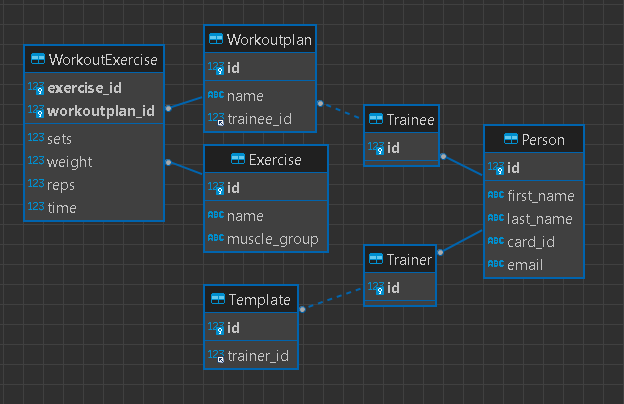
\includegraphics[width=1\textwidth]{pics/erd.png}
    \caption{ERD der Datenbankstruktur}
    \label{fig:erd}
\end{figure}
\newpage

\subsection{Datenbankverbindung für IntelliJ Projekt}
\begin{lstlisting}[language=Java,caption=Datenbank verbindung,label=lst:impl:foo]
    # Configuration file

    quarkus.swagger-ui.path=/swagger
    quarkus.swagger-ui.always-include=true
    
    # MS SQL DB connection
    quarkus.datasource.db-kind=mysql
    quarkus.datasource.username=****
    quarkus.datasource.password=***************
    quarkus.datasource.jdbc.url=jdbc:mysql://localhost:3306/AberGymDb
    #quarkus.hibernate-orm.database.generation=drop-and-create
    quarkus.hibernate-orm.database.generation=create
    #quarkus.hibernate-orm.database.generation=update
    #quarkus.hibernate-orm.sql-load-script=import.sql
\end{lstlisting}

Dieser Code zeigt die Konfigurationsdatei des Trainingsplan-Verwaltungssystems. Die Konfigurationsdatei legt die Einstellungen und Parameter fest, die das System beeinflussen. Die ersten beiden Einträge definieren den Pfad und die Verfügbarkeit der Swagger-UI, die eine grafische Benutzeroberfläche bietet, um das System zu testen und zu dokumentieren.
\newline
\newline
Die nächsten Einträge definieren die Verbindung zu einer MySQL-Datenbank. Der Befehl "quarkus.datasource.db-kind" gibt an, welcher Typ von Datenbank verwendet wird, in diesem Fall MySQL. "quarkus.datasource.username" und "quarkus.datasource.password" legen die Anmeldeinformationen für den Zugriff auf die Datenbank fest. "quarkus.datasource.jdbc.url" gibt die URL an, unter der die Datenbank erreichbar ist.
\newline
\newline
Der nächste Eintrag "quarkus.hibernate-orm.database.generation" gibt an, wie die Datenbank erstellt werden soll. In diesem Fall wird die Datenbank jedes Mal, wenn die Anwendung gestartet wird, erstellt, indem der Befehl "create" verwendet wird. Alternativ könnte der Befehl "update" verwendet werden, um die Datenbank zu aktualisieren, oder "drop-and-create", um die Datenbank vollständig zu löschen und neu zu erstellen.
\newline
\newline
Der letzte Eintrag "quarkus.hibernate-orm.sql-load-script" gibt an, welches SQL-Skript verwendet werden soll, um Daten in die Datenbank zu importieren. In diesem Fall wird kein Skript verwendet.
\newline
\newline
Die Konfigurationsdatei ist ein wichtiger Bestandteil des Trainingsplan-Verwaltungssystems, da sie die Verbindung zur Datenbank und die Erstellung der Datenbank definiert. Durch die Verwendung von Quarkus und Hibernate können Entwickler*innen schnell und einfach Datenbankanwendungen erstellen und konfigurieren.

\subsection{Demodaten für den Entwicklungsprozess der Mobile Anwendung}
\setauthor{Antonio Peric}  

Der Befehl "INSERT INTO" ist ein grundlegender SQL-Befehl, der verwendet wird, um neue Datensätze in eine Datenbanktabelle einzufügen. Mit diesem Befehl können Daten in eine Tabelle eingefügt werden, indem der Befehl "VALUES" verwendet wird, um die Werte für die einzelnen Spalten anzugeben.
\newline
\newline
Die Syntax des Befehls "INSERT INTO" lautet wie folgt:

\begin{verbatim}
    INSERT INTO table_name (column1, column2, column3, ...)
    VALUES (value1, value2, value3, ...);
\end{verbatim}


Der Befehl beginnt mit dem Namen der Tabelle, in die die Daten eingefügt werden sollen. Anschließend werden in Klammern die Namen der Spalten angegeben, in die die Daten eingefügt werden sollen. Wenn der Befehl "INSERT INTO" verwendet wird, um in alle Spalten einer Tabelle einzufügen, kann die Angabe von Spaltennamen entfallen.
\newline
\newline
Die Werte, die in die Tabelle eingefügt werden sollen, werden nach dem Befehl "VALUES" aufgelistet und durch Kommas getrennt. Die Reihenfolge der Werte muss mit der Reihenfolge der Spaltennamen übereinstimmen.
\newline
\newline
Ein Beispiel für die Verwendung des Befehls "INSERT INTO" lautet wie folgt:
\begin{verbatim}
    INSERT INTO customers (name, address, city, state, zip)
    VALUES ('Max Mustermann', 'Musterstraße 1', 'Musterstadt', 'Musterland', '12345');
\end{verbatim}


In diesem Beispiel wird ein neuer Datensatz in die Tabelle "customers" eingefügt. Der Datensatz enthält die Werte "Max Mustermann" für den Namen, "Musterstraße 1" für die Adresse, "Musterstadt" für die Stadt, "Musterland" für den Staat und "12345" für die Postleitzahl.
\newline
\newline
Der Befehl "INSERT INTO" ist ein wichtiger Bestandteil der Datenmanipulation in SQL und wird häufig in Kombination mit anderen Befehlen wie "SELECT", "UPDATE" und "DELETE" verwendet, um Daten in einer Datenbank zu verwalten.
\newpage

\subsection{Import Datei für die Demo Daten}

\begin{verbatim}
    --------------------------------------------------------
    --  First Customer | Test data
    --------------------------------------------------------
    Insert into Person (first_name,last_name,email,cardId) 
        values ('Antonio','Peric','test@gmail.com','**************');
    Insert into Trainee (id) values (1);
    
    --------------------------------------------------------
    --  First Workoutplan
    --------------------------------------------------------
    
    Insert into Workoutplan (name,trainee_id) 
        values ('Ganzkörper Workout', 1);
    
    --  Exercise
    
    Insert into Exercise (name) values ('Liegestütze');
    Insert into Exercise (name) values ('Bench Press');
    Insert into Exercise (name) values ('Cable Flys');
    Insert into Exercise (name) values ('Incline Dumbell press');
    Insert into Exercise (name) values ('Biceps Curls');
    Insert into Exercise (name) values ('Triceps Extension');
    Insert into Exercise (name) values ('Triceps Curls');
    Insert into Exercise (name) values ('Skullcrusher');
    
    -- WorkoutExercise
    
    Insert into WorkoutExercise (sets,weight,reps,workoutplan_id, exercise_id) 
        values (5,0.0,50,1,1);
    Insert into WorkoutExercise (sets,weight,reps,workoutplan_id, exercise_id) 
        values (3,100.0,6,1,2);
    Insert into WorkoutExercise (sets,weight,reps,workoutplan_id, exercise_id) 
        values (3,20.0,25,1,3);
    Insert into WorkoutExercise (sets,weight,reps,workoutplan_id, exercise_id) 
        values (3,32.5,15,1,4);
    Insert into WorkoutExercise (sets,weight,reps,workoutplan_id, exercise_id) 
        values (5,12.5,15,1,5);
    Insert into WorkoutExercise (sets,weight,reps,workoutplan_id, exercise_id) 
        values (5,80.5,20,1,6);
    Insert into WorkoutExercise (sets,weight,reps,workoutplan_id, exercise_id) 
        values (2,80.0,20,1,7);
    Insert into WorkoutExercise (sets,weight,reps,workoutplan_id, exercise_id) 
        values (4,30.0,20,1,8);
    
    --------------------------------------------------------
    --  Second Workoutplan
    --------------------------------------------------------
    
    Insert into Workoutplan (name,trainee_id) values ('Ganzkörper Workout', 1);
    
    -- WorkoutExercise
    
    Insert into WorkoutExercise (sets,weight,reps,workoutplan_id, exercise_id) 
        values (5,10,50,2,1);
    Insert into WorkoutExercise (sets,weight,reps,workoutplan_id, exercise_id) 
        values (3,100.0,6,2,2);
    Insert into WorkoutExercise (sets,weight,reps,workoutplan_id, exercise_id) 
        values (3,20.0,25,2,3);
    Insert into WorkoutExercise (sets,weight,reps,workoutplan_id, exercise_id) 
        values (3,32.5,15,2,4);
    Insert into WorkoutExercise (sets,weight,reps,workoutplan_id, exercise_id) 
        values (5,12.5,15,2,5);
    Insert into WorkoutExercise (sets,weight,reps,workoutplan_id, exercise_id) 
        values (5,80.5,20,2,6);
    Insert into WorkoutExercise (sets,weight,reps,workoutplan_id, exercise_id) 
        values (2,80.0,20,2,7);
    Insert into WorkoutExercise (sets,weight,reps,workoutplan_id, exercise_id) 
        values (4,30.0,20,2,8);
\end{verbatim}
\newpage
Der bereitgestellte Code enthält SQL-Anweisungen, die in eine MySQL-Datenbank eingefügt werden sollen. Der erste Teil des Codes bezieht sich auf die Testdaten des ersten Kunden*inn und besteht aus zwei Insert-Anweisungen, die Daten in die Tabellen Person und Trainee einfügen.
\newline
\newline
Der zweite Teil des Codes bezieht sich auf den ersten Trainingsplan, der erstellt wird. Die Insert-Anweisung fügt einen neuen Eintrag in die Workoutplan-Tabelle ein und weist ihn dem Trainee mit der ID 1 zu.
\newline
\newline
Der dritte Teil des Codes bezieht sich auf die einzelnen Übungen, die Teil des Trainingsplans sind. Die Insert-Anweisungen fügen neue Einträge in die Exercise-Tabelle ein.
\newline
\newline
Der letzte Teil des Codes fügt die einzelnen Übungen mit den entsprechenden Sets, Gewichten und Wiederholungen in die WorkoutExercise-Tabelle ein und weist sie dem ersten Trainingsplan zu. Es werden auch Insert-Anweisungen für den zweiten Trainingsplan erstellt, die die gleichen Übungen wie der erste Trainingsplan enthalten, jedoch unterschiedliche Set-, Gewichts- und Wiederholungswerte aufweisen.
\newpage

\section{Integration des echten Backends}
\setauthor{Antonio Peric} 

\subsection{LeoCloud}
LeoCloud ist ein Kubernetes Cluster, der von der HTBLA Leonding betrieben wird und Schülern zur Verfügung steht. Kubernetes ist eine Container-Orchestrierungsplattform, die es Entwicklern ermöglicht, Containeranwendungen effizient zu erstellen, zu verwalten und zu skalieren. LeoCloud stellt Schülern eine Umgebung zur Verfügung, um praktische Erfahrungen mit der Container-Technologie und der Entwicklung von Cloud-Anwendungen zu sammeln.
\newline
\newline
Das Backend des Projekts AberGym-Syp wird auf LeoCloud gehostet, was den Entwicklern eine zuverlässige und skalierbare Plattform bietet, um die Anwendung bereitzustellen. Die Nutzung von Kubernetes ermöglicht eine automatisierte Skalierung von Ressourcen, die die Anforderungen der Anwendung erfüllen. So kann die Leistungsfähigkeit des Backends bei Bedarf erhöht werden, ohne manuelle Eingriffe von Seiten des Entwicklers.
\newline
\newline
Die Integration von Rest-Schnittstellen ermöglicht es, auf die Datenbank des Projekts AberGym-Syp zuzugreifen. Die MySql-Datenbank enthält alle relevanten Informationen, die von der Anwendung benötigt werden, um die Trainingspläne zu erstellen und zu verwalten. Das Einrichten von Rest-Schnittstellen erleichtert den Datenaustausch zwischen verschiedenen Anwendungen und ermöglicht eine einfache Integration in andere Systeme.
\newline
\newline
Die Nutzung von LeoCloud und Kubernetes ist ein Beispiel für den Einsatz moderner Cloud-Technologien in der Bildung. Es bietet Schülern eine Plattform, um praktische Erfahrungen mit den neuesten Technologien zu sammeln und ihre Fähigkeiten in der Entwicklung von Cloud-Anwendungen zu verbessern.